\documentclass[a4paper,12pt]{article} 

%%% Работа с русским языком
\usepackage{cmap}					% поиск в PDF
\usepackage{mathtext} 				% русские буквы в фомулах
\usepackage[T2A]{fontenc}			% кодировка
\usepackage[utf8]{inputenc}			% кодировка исходного текста
\usepackage[english,russian]{babel}	% локализация и переносы

%%% Дополнительная работа с математикой
\usepackage{amsmath,amsfonts,amssymb,amsthm,mathtools, gensymb} % AMS
\usepackage{icomma} % "Умная" запятая: $0,2$    ф--- число, $0, 2$ --- перечисление

%%Таблица
\usepackage[table,xcdraw]{xcolor}
\usepackage{caption}
\usepackage{floatrow}
\floatsetup[table]{capposition=top}
\floatsetup[wrapfigure]{capposition=bottom}
\usepackage{multirow}

\usepackage{hyperref}

%Отступы и поля 
\textwidth=18cm
\oddsidemargin=-1cm
\topmargin=-2cm
\textheight=25cm


%% Номера формул
\mathtoolsset{showonlyrefs=false} % Показывать номера только у тех формул, на которые есть \ref{} в тексте.

%% Шрифты
\usepackage{euscript}	 % Шрифт Евклид
\usepackage{mathrsfs} % Красивый матшрифт

%% Свои команды
\DeclareMathOperator{\sgn}{\mathop{sgn}}

%% Перенос знаков в формулах (по Львовскому)
\newcommand*{\hm}[1]{#1\nobreak\discretionary{}
{\hbox{$\mathsurround=0pt #1$}}{}}

%% Стиль страницы
\usepackage{fancyhdr}

%% Для рисунков
\usepackage{graphicx}
\usepackage[export]{adjustbox}
\usepackage{float}
\usepackage{ragged2e}
\usepackage{wrapfig}

\pagestyle{fancy}
\begin{document}
\begin{titlepage}
\begin{center}
%\vspace*{1cm}
\large{\small ФЕДЕРАЛЬНОЕ ГОСУДАРСТВЕННОЕ АВТОНОМНОЕ ОБРАЗОВАТЕЛЬНОЕ\\ УЧРЕЖДЕНИЕ ВЫСШЕГО ОБРАЗОВАНИЯ \\ МОСКОВСКИЙ ФИЗИКО-ТЕХНИЧЕСКИЙ ИНСТИТУТ\\ (НАЦИОНАЛЬНЫЙ ИССЛЕДОВАТЕЛЬСКИЙ УНИВЕРСИТЕТ)\\ ФАКУЛЬТЕТ АЭРОКОСМИЧЕСКИХ ТЕХНОЛОГИЙ}
\vfill
\line(1,0){490}\\[1mm]
\huge{Лабораторная работа 5.5}\\
\huge\textbf{Компьютерная сцинтилляционная $\gamma$-спектрометрия}\\
\line(1,0){490}\\[1mm]
\vfill
\begin{flushright}
\normalsize{Рогозин Владимир}\\
\normalsize{\textbf{Группа Б03-106}}\\
\end{flushright}
\end{center}
\end{titlepage}
\fancyhead[L] {Работа 5.5}

\textbf{Цель работы}:
определение энергии и интенсивности дискретных гамма-линий от различных гамма-источников и их идентификация.


% \textbf{Оборудование}:
% лазер; кассета с набором сеток разного
% периода; линзы; щель с микрометрическим винтом; оптический стол
% c набором рейтеров и крепёжных винтов; экран; линейка.


\section{Теоретические сведения}
Основная задача спектрометрических измерений заключается в определении энергии и интенсивности дискретных гамма-линий от различных гамма-источников и их идентификации.

В данной работе исследуются сцинтилляционные гамма-спектрометры на
основе неорганического кристалла NaI(Tl).

При прохождении гамма-квантов через материальную среду образуются электроны, возникающие за счет фотоэффекта, комптоновского рассеяния и рождения электрон-позитронных пар. Неупругие соударения могут сопровождаться как ионизацией, так и
возбуждением молекул или атомов среды. На промежуточных же стадиях (при переходах возбужденных молекул или атомов в основное состояние, при рекомбинации электрических зарядов и т.п.) в веществе возникают кванты света различных длин волн, присущих данному веществу.

Вообще говоря, возникающее излучение должно сильно поглощаться в сцинтилляторе, так как его энергия в точности равна энергии возбуждения атомов среды. Чтобы избежать этого явления, в кристаллы сцинтиллятора вводят небольшие добавки других атомов. Свободные локальные уровни энергии электрона на примесных атомах таллия располагаются внутри запрещенной зоны кристалла NaI. В процессе релаксации возможны переходы электронов, возбужденных в зону проводимости, на эти уровни. Энергии излучаемых при таких переходах фотонов меньше ширины запрещенной зоны, и они могут поглощаться только атомами таллия. Но концентрация таллия мала (порядка $0,1\%$), поэтому мало поглощение указанных фотонов, и они имеют все шансы вылететь из сцинтиллятора. В этом случае прохождение ионизирующей частицы через вещество будет сопровождаться световой вспышкой, которая и может быть использована для регистрации частицы.

Cовременный сцинтилляционный счетчик состоит из сцинтиллятора -- вещества, способного испускать видимое или ультрафиолетовое излучение, возникающее под действием заряженных частиц, и фотоэлектронного умножителя, в котором энергия этих световых вспышек через посредство фотоэффекта преобразуется в импульсы электрического тока.

\subsection{Процессы взаимодействия гамма-излучения с веществом}
Основными процессами взаимодействия гамма-излучения с веществом являются, как было выше указано, фотоэффект, эффект Комптона и образование электрон-позитронных пар. Каждый из этих процессов вносит свой вклад в образование наблюдаемого спектра.

\textbf{Фотоэффект} -- процесс взаимодействия гамма-кванта с электроном, связанным с атомом, при котором электрону передается вся энергия гамма-кванта. При этом электрону сообщается кинетическая энергия $T_e = E_\gamma - I_i$, где $E_\gamma$ -- энергия гамма-кванта, $I_i$ -- потенциал ионизации $i$-той оболочки атома. Фотоэффект особенно существенен для тяжелых веществ, где он идет с заметной вероятностью даже при высоких энергиях гамма-квантов. В легких
веществах фотоэффект становится заметен лишь при относительно небольших энергиях гамма-квантов.

\textbf{Эффект Комптона} -- упругое рассеяние фотона на свободном электроне,
сопровождающееся изменением длины волны фотона (реально этот процесс происходит на слабо связанных с атомом внешних электронах). Максимальная энергия образующихся комптоновских электронов соответствует рассеянию гамма-квантов на $180\degree$ и равна
\begin{equation}\label{eq: Compton E_max}
    E_{max} = \frac{\hbar \omega}{1 + \frac{2\hbar \omega}{mc^2}}.
\end{equation}

\textbf{Процесс образования электрон-позитронных пар.} При достаточно высокой энергии гамма-кванта наряду с фотоэффектом и эффектом Комптона может происходить третий вид взаимодействия гамма-квантов с веществом -- образование электрон-позитронных пар. Процесс образования пар не может происходить в пустоте, так как в этом случае не выполняются совместно законы сохранения энергии и импульса. В присутствии ядра или электрона процесс образования пары гамма-квантом возможен, так как можно распределить энергию и импульс гамма-кванта между тремя частицами без противоречия с законами сохранения. При этом если процесс образования пары
идет в кулоновском поле ядра, то энергия образующегося ядра отдачи оказывается весьма малой, так что пороговая энергия гамма-кванта $E_\text{пор}$, необходимая для образования пары, практически совпадает с удвоенной энергией покоя электрона $E_\text{пор} \approx 2mc^2 = 1,022$ МэВ.

Появившиеся в результате процесса образования пар частицы теряют свою кинетическую энергию на ионизацию среды. Таким образом, вся энергия электрона остается в детекторе. Позитрон будет двигаться до тех пор, пока практически не остановится, а затем аннигилирует с электроном среды, в результате чего появятся два гамма-кванта. Т.е., кинетическая энергия позитрона также останется в детекторе. Далее возможны три варианта развития событий: \par
a) оба родившихся гамма-кванта не вылетают из детектора, и тогда вся энергия первичного гамма-кванта останется в детекторе, а в спектре появится пик с $E = E_\gamma$; \par
б) один из родившихся гамма-квантов покидает детектор, и в спектре появляется пик, соответствующий энергии $E = E_\gamma - E_0$, где $E_0= mc^2 = 511$ кэВ; \par
в) оба родившихся гамма-кванта покидают детектор, и в спектре появляется пик, соответствующий энергии $E = E_\gamma - 2E_0$, где $2E_0= 2mc^2 = 1022$ кэВ. \par

Таким образом, любой спектр, получаемый с помощью гамма-спектрометра, описывается несколькими компонентами, каждая из которых связана с определенным физическим процессом. Каждый процесс взаимодействия гамма-квантов с веществом вносит свой вклад в образование спектра. Помимо этих процессов, добавляются экспонента, связанная с наличием фона, пик характеристического излучения, возникающий при взаимодействии гамма-квантов с окружающим веществом, а также пик обратного рассеяния, образующийся при энергии квантов $E_\gamma \gg mc^2$ в результате рассеяния гамма-квантов на большие углы на материалах конструктивных элементов детектора и защиты и последующего фотоэффекта в сцинтилляторе. Положение пика обратного рассеяния определяется по формуле (\ref{eq: Compton E_max})

\section{Экспериментальная установка}
Принципиальная блок-схема гамма-спектрометра, изучаемого в данной
работе, показана на рис. \hyperref[fig: Exp setup]{1}.
\begin{figure}[H]\label{fig: Exp setup}
    \centering
    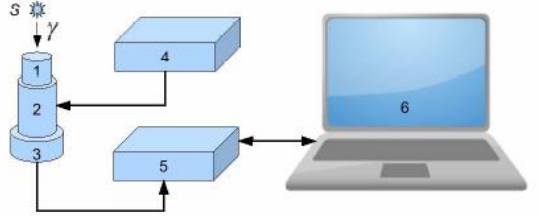
\includegraphics[width = 0.51\textwidth]{Exp setup.png}
    \caption{Принципиальная блок-схема спектрометра. (1 -- сцинтиллятор, 2 --       ФЭУ, 3 -- предусилитель импульсов, 4 -- высоковольтный блок питания для       ФЭУ, 5 -- блок преобразования аналоговых импульсов с ФЭУ в цифровой код       (АЦП), 6 -- компьютер для сбора данных, их обработки и хранения).}
\end{figure}

ФЭУ со сцинтиллятором и блоком питания установлены на отдельной подставке. В нашей работе на разных установках в качестве сцинтиллятора используются кристаллы NaI(Tl) с размерами $\varnothing$ $45\times50$ мм и $\varnothing$ $20\times25$ мм.


\section{Обработка данных}

\subsection{Проверка функционирования установки}
\begin{enumerate}
    \item
    Включим измерительные устройства и компьютер, запустим программу и войдём в режим измерения спектра. Проверим функционирование установки в этом режиме: при увеличении угла отклонения фотопик должен смещаться влево, в сторону меньших энергий.
    \item 
    Подберём напряжение так, чтобы при нулевом угле $\theta =0\degree$ фотопик был смещен на экране максимально вправо. Дальнейшие измерения были проведены при напряжении $V = 1,2$ В.
\end{enumerate}

\subsection{Калибровка зависимости номера канала от энергии}
\begin{enumerate}
    \item
    По известным значениям энергии поглощения для Co, Na и Cs построим линейную аппроксимацию зависимости номера канала $N$ от соответствующей ему энергии $E$.
    \begin{table}[H]\label{tab: NE}
        \centering
        \begin{tabular}{|
            >{\columncolor[HTML]{FFFFFF}}c |
            >{\columncolor[HTML]{FFFFFF}}c 
            >{\columncolor[HTML]{FFFFFF}}c |
            >{\columncolor[HTML]{FFFFFF}}c 
            >{\columncolor[HTML]{FFFFFF}}c |
            >{\columncolor[HTML]{FFFFFF}}c |}
            \hline
            {\color[HTML]{000000} } &
              \multicolumn{2}{c|}{\cellcolor[HTML]{FFFFFF}{\color[HTML]{000000} Co}} &
              \multicolumn{2}{c|}{\cellcolor[HTML]{FFFFFF}{\color[HTML]{000000} Na}} &
              {\color[HTML]{000000} Cs} \\ \hline
            {\color[HTML]{000000} $E$, кэВ} &
              \multicolumn{1}{c|}{\cellcolor[HTML]{FFFFFF}{\color[HTML]{000000} $1173,2$}} &
              {\color[HTML]{000000} $1332,5$} &
              \multicolumn{1}{c|}{\cellcolor[HTML]{FFFFFF}{\color[HTML]{000000} $511$}} &
              {\color[HTML]{000000} $1274$} &
              {\color[HTML]{000000} $661,7$} \\ \hline
            {\color[HTML]{000000} $N$, номер канала} &
              \multicolumn{1}{c|}{\cellcolor[HTML]{FFFFFF}{\color[HTML]{000000} 1570}} &
              {\color[HTML]{000000} 1800} &
              \multicolumn{1}{c|}{\cellcolor[HTML]{FFFFFF}{\color[HTML]{000000} 700}} &
              {\color[HTML]{000000} 1730} &
              {\color[HTML]{000000} 900} \\ \hline
        \end{tabular}
        \caption{Номера канала и соответствующие им энергии}
    \end{table}
\end{enumerate}

\subsection{Вычисление энергетического разрешения}
\begin{enumerate}
    \item 
    Определим энергетическое разрешения для каждого измерения по формуле \fbox{$R_i = \frac{\Delta E_i}{E_i}$}. Для перехода от номера канала к энергии будем использовать результат предыдущего пункта.
    \begin{table}[H]\label{tab: R}
        \centering
        \begin{tabular}{|
        >{\columncolor[HTML]{FFFFFF}}c |
        >{\columncolor[HTML]{FFFFFF}}c |
        >{\columncolor[HTML]{FFFFFF}}c |
        >{\columncolor[HTML]{FFFFFF}}c |
        >{\columncolor[HTML]{FFFFFF}}c |
        >{\columncolor[HTML]{FFFFFF}}c |}
        \hline
        {\color[HTML]{000000} Источник} &
          {\color[HTML]{000000} $N_i$} &
          {\color[HTML]{000000} $\Delta N_i$} &
          {\color[HTML]{000000} $E_i$, кэВ} &
          {\color[HTML]{000000} $\Delta E_i$, кэВ} &
          {\color[HTML]{000000} $R_i$} \\ \hline
        \cellcolor[HTML]{FFFFFF}{\color[HTML]{000000} } &
          {\color[HTML]{000000} 1570} &
          {\color[HTML]{000000} 76,5} &
          {\color[HTML]{000000} 1162,3} &
          {\color[HTML]{000000} 102,4} &
          {\color[HTML]{000000} 0,09} \\ \cline{2-6} 
        \multirow{-2}{*}{\cellcolor[HTML]{FFFFFF}{\color[HTML]{000000} Co}} &
          {\color[HTML]{000000} 1800} &
          {\color[HTML]{000000} 82,1} &
          {\color[HTML]{000000} 1334,1} &
          {\color[HTML]{000000} 109,9} &
          {\color[HTML]{000000} 0,08} \\ \hline
        \cellcolor[HTML]{FFFFFF}{\color[HTML]{000000} } &
          {\color[HTML]{000000} 700} &
          {\color[HTML]{000000} 50,1} &
          {\color[HTML]{000000} 512,5} &
          {\color[HTML]{000000} 67,1} &
          {\color[HTML]{000000} 0,13} \\ \cline{2-6} 
        \multirow{-2}{*}{\cellcolor[HTML]{FFFFFF}{\color[HTML]{000000} Na}} &
          {\color[HTML]{000000} 1730} &
          {\color[HTML]{000000} 80,1} &
          {\color[HTML]{000000} 1281,7} &
          {\color[HTML]{000000} 107,2} &
          {\color[HTML]{000000} 0,08} \\ \hline
        {\color[HTML]{000000} Cs} &
          {\color[HTML]{000000} 900} &
          {\color[HTML]{000000} 58,2} &
          {\color[HTML]{000000} 661,8} &
          {\color[HTML]{000000} 77,9} &
          {\color[HTML]{000000} 0,12} \\ \hline
        \cellcolor[HTML]{FFFFFF}{\color[HTML]{000000} } &
          {\color[HTML]{000000} 1905} &
          {\color[HTML]{000000} 86,2} &
          {\color[HTML]{000000} 1412, 5} &
          {\color[HTML]{000000} 115,4} &
          {\color[HTML]{000000} 0,08} \\ \cline{2-6} 
        \cellcolor[HTML]{FFFFFF}{\color[HTML]{000000} } &
          {\color[HTML]{000000} 1490} &
          {\color[HTML]{000000} 116,4} &
          {\color[HTML]{000000} 1102,5} &
          {\color[HTML]{000000} 155,8} &
          {\color[HTML]{000000} 0,14} \\ \cline{2-6} 
        \cellcolor[HTML]{FFFFFF}{\color[HTML]{000000} } &
          {\color[HTML]{000000} 1054} &
          {\color[HTML]{000000} 64,8} &
          {\color[HTML]{000000} 777,2} &
          {\color[HTML]{000000} 86,8} &
          {\color[HTML]{000000} 0,11} \\ \cline{2-6} 
        \cellcolor[HTML]{FFFFFF}{\color[HTML]{000000} } &
          {\color[HTML]{000000} 474} &
          {\color[HTML]{000000} 37,5} &
          {\color[HTML]{000000} 343,8} &
          {\color[HTML]{000000} 50,2} &
          {\color[HTML]{000000} 0,15} \\ \cline{2-6} 
        \cellcolor[HTML]{FFFFFF}{\color[HTML]{000000} } &
          {\color[HTML]{000000} 342} &
          {\color[HTML]{000000} 29,7} &
          {\color[HTML]{000000} 244,8} &
          {\color[HTML]{000000} 39,8} &
          {\color[HTML]{000000} 0,16} \\ \cline{2-6} 
        \multirow{-6}{*}{\cellcolor[HTML]{FFFFFF}{\color[HTML]{000000} Eu}} &
          {\color[HTML]{000000} 241} &
          {\color[HTML]{000000} 23,7} &
          {\color[HTML]{000000} 169,9} &
          {\color[HTML]{000000} 31,7} &
          {\color[HTML]{000000} 0,19} \\ \hline
        \cellcolor[HTML]{FFFFFF}{\color[HTML]{000000} } &
          {\color[HTML]{000000} 97} &
          {\color[HTML]{000000} 10,1} &
          {\color[HTML]{000000} 61,9} &
          {\color[HTML]{000000} 13,5} &
          {\color[HTML]{000000} 0,22} \\ \cline{2-6} 
        \multirow{-2}{*}{\cellcolor[HTML]{FFFFFF}{\color[HTML]{000000} Am}} &
          {\color[HTML]{000000} 50} &
          {\color[HTML]{000000} 13,0} &
          {\color[HTML]{000000} 26,7} &
          {\color[HTML]{000000} 17,4} &
          {\color[HTML]{000000} 0,65} \\ \hline
        \end{tabular}
        \caption{Результаты вычисления  энергетического разрешения}
    \end{table}  
\end{enumerate}

\subsection{Вычисление края комптоновского рассеяния}
\begin{enumerate}
    \item 
    Занесём в таблицу номер канал и теоретическое значение энергии, соответствующего максимума энергии комптоновского рассеяния.
    \begin{table}[H]\label{tab: comptE data}
        \centering
        \begin{tabular}{|
            >{\columncolor[HTML]{FFFFFF}}c |
            >{\columncolor[HTML]{FFFFFF}}c |
            >{\columncolor[HTML]{FFFFFF}}c 
            >{\columncolor[HTML]{FFFFFF}}c |
            >{\columncolor[HTML]{FFFFFF}}c |}
            \hline
            {\color[HTML]{000000} } &
              {\color[HTML]{000000} Co} &
              \multicolumn{2}{c|}{\cellcolor[HTML]{FFFFFF}{\color[HTML]{000000} Na}} &
              {\color[HTML]{000000} Cs} \\ \hline
            {\color[HTML]{000000} $E_\gamma$, кэВ} &
              {\color[HTML]{000000} 1173,2} &
              \multicolumn{1}{c|}{\cellcolor[HTML]{FFFFFF}{\color[HTML]{000000} 511}} &
              {\color[HTML]{000000} 1274} &
              {\color[HTML]{000000} 661,7} \\ \hline
            {\color[HTML]{000000} $N_i$} &
              {\color[HTML]{000000} 1200} &
              \multicolumn{1}{c|}{\cellcolor[HTML]{FFFFFF}{\color[HTML]{000000} 350}} &
              {\color[HTML]{000000} 1300} &
              {\color[HTML]{000000} 625} \\ \hline
        \end{tabular}
        \caption{Данные для изучения энергетической границы комптоновского                эффекта}
    \end{table}
\end{enumerate}

\section{Вывод}
В данной работе исследовался принцип работы сцинтиллятора. В результате удалось:
\begin{itemize}
    \item
    получить спектры излучения для Co, Cs, Na, Eu и Am.
    
    \item
    выделить отдельные части спектра, отвечающие за фотоэффект, эффект Комптона, обратное рассеяние и характеристическое излучение свинца.

    \item
    измерить энергетическую разрешение, результат с плохой точностью совпал с теорией.  
    
\end{itemize}

\newpage
%%%%%%%%%%%%%%%%%%%%%%%%% Графики
\begin{figure}[H]\label{fig: N(E)}
    \centering
    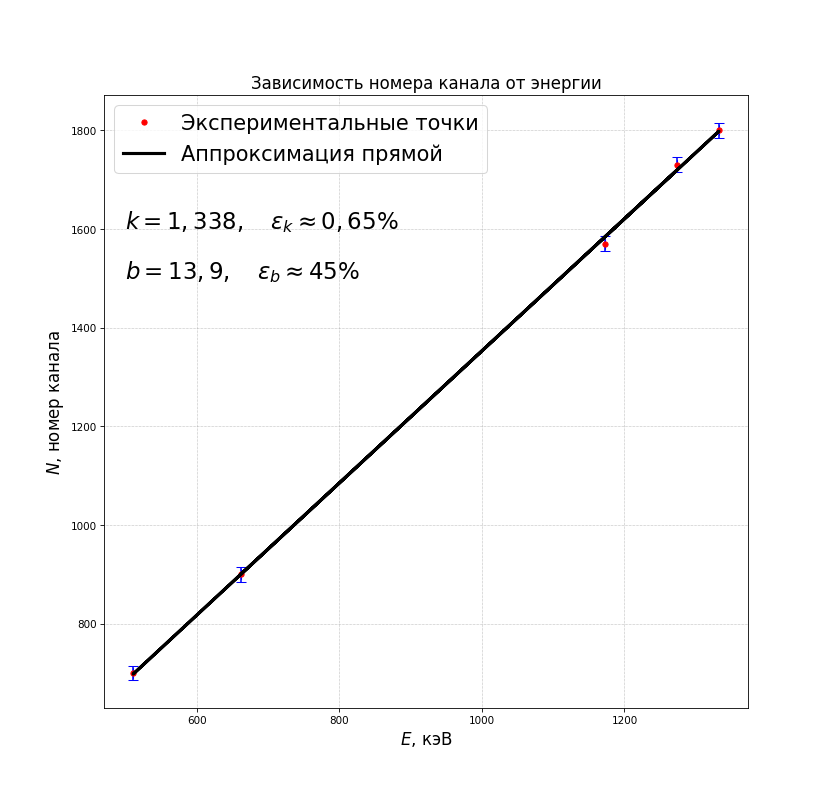
\includegraphics[width = \textwidth]{N(E).png}
\end{figure}
\[k = (1,338 \pm 0,009)\text{ 1/кэВ}, \quad \varepsilon_k \approx 0,65 \%,\]
\[b = 13,9 \pm 6,3, \quad \varepsilon_b \approx 45 \%.\]
\newpage

\begin{figure}[H]\label{fig: RR(E-1)}
    \centering
    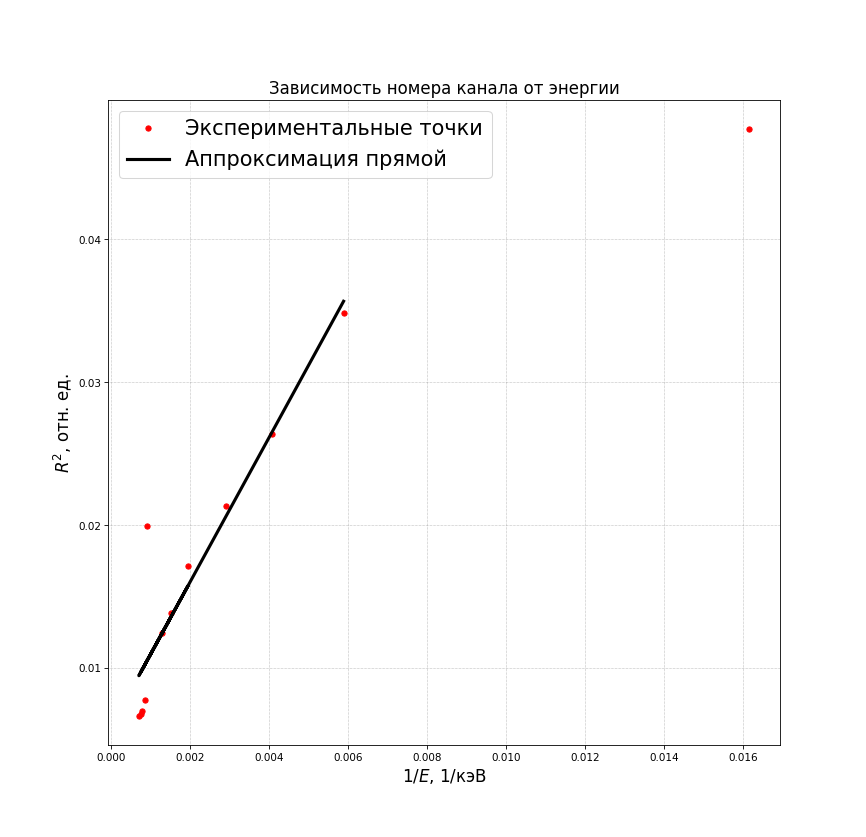
\includegraphics[width = \textwidth]{RR(E-1).png}
\end{figure}
\[k = (5,06 \pm 0,7)\text{ кэВ}, \quad \varepsilon_k \approx 14 \%,\]
\[b = (6,0 \pm 1,8)\cdot 10^{-3}, \quad \varepsilon_b \approx 29 \%.\]
\newpage

\begin{figure}[H]\label{fig: Ecompt(Egamma)}
    \centering
    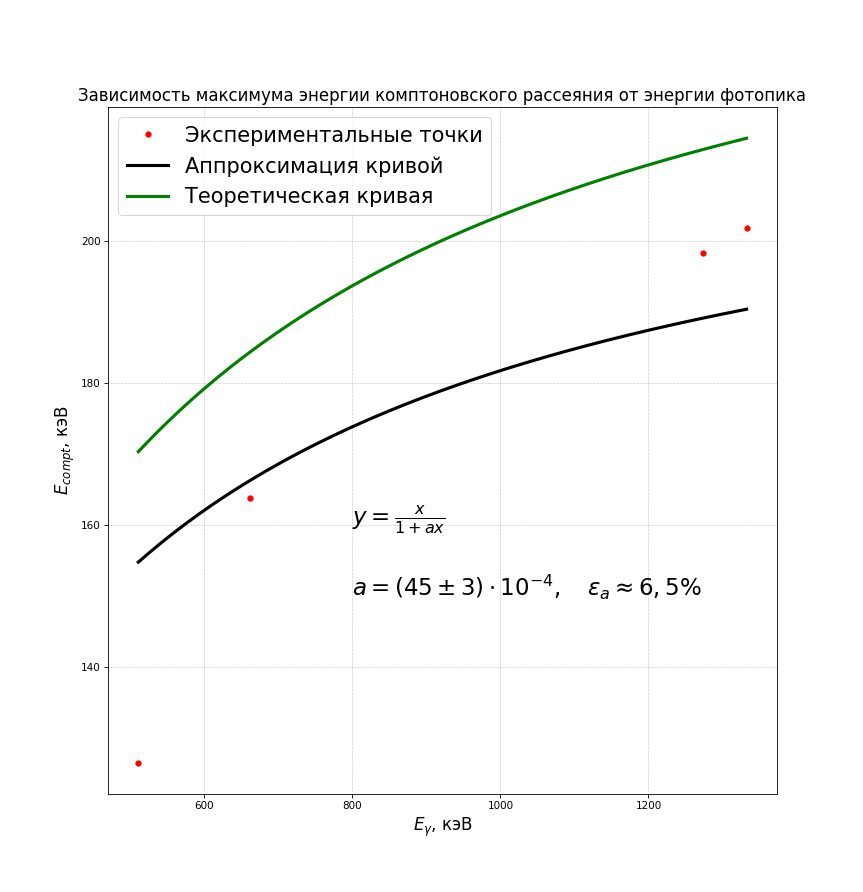
\includegraphics[width = \textwidth]{Ecompt(Egamma).png}
\end{figure}
\newpage



%%%%%%%%%%%%%%%%%%%%%%%%%
\end{document}
